\documentclass[11pt,a4paper]{report}

% ---- Encoding & font ----------------------------------------
\usepackage[T1]{fontenc}
\usepackage[utf8]{inputenc}
\usepackage{lmodern}           % Latin Modern: clean, breathes well

% ---- Page geometry ------------------------------------------
\usepackage[
  top=2.5cm, bottom=3.0cm,
  left=3.0cm, right=2.8cm,
  headheight=15pt
]{geometry}

% ---- Spacing ------------------------------------------------
\usepackage{setspace}
\setlength{\parindent}{0pt}
\setlength{\parskip}{0.55em}
\linespread{1.12}

% ---- Core packages ------------------------------------------
\usepackage{xcolor}
\usepackage{graphicx}
\usepackage{booktabs}
\usepackage{tabularx}
\usepackage{array}
\usepackage{enumitem}
\usepackage{microtype}
\usepackage{amsmath}
\usepackage{amssymb}
\usepackage{float}
\usepackage{caption}
\usepackage{tcolorbox}
\tcbuselibrary{skins, breakable}

% ---- Colors -------------------------------------------------
\definecolor{primary}{RGB}{45, 106, 79}       % deep emerald (headings)
\definecolor{secondary}{RGB}{39, 170, 130}    % teal (sub-headings, rules)
\definecolor{accent}{RGB}{220, 100, 30}       % warm orange (tags, callouts)
\definecolor{dark}{RGB}{22, 28, 36}           % near-black body
\definecolor{light}{RGB}{245, 250, 247}       % near-white page tint

% Code block palette (VSCode dark)
\definecolor{codebg}{RGB}{30, 30, 46}
\definecolor{codefg}{RGB}{205, 214, 244}
\definecolor{codekw}{RGB}{137, 180, 250}
\definecolor{codestr}{RGB}{166, 227, 161}
\definecolor{codecmt}{RGB}{108, 112, 134}
\definecolor{codenum}{RGB}{250, 179, 135}

% Inline tag palette
\definecolor{tagUI}{RGB}{45, 106, 79}
\definecolor{tagAGG}{RGB}{39, 170, 130}
\definecolor{tagDEC}{RGB}{220, 100, 30}
\definecolor{tagREJ}{RGB}{100, 100, 115}
\definecolor{tagGAP}{RGB}{180, 30, 50}
\definecolor{tagNOV}{RGB}{60, 130, 190}
\definecolor{tagDATA}{RGB}{130, 80, 180}
\definecolor{tagTEST}{RGB}{39, 150, 100}

% ---- Tag macros ---------------------------------------------
% [UI], [AGG], [DEC] etc rendered as small-caps colored bracketed label
% No border box. Just tight colored text in brackets.
\newcommand{\taglabel}[2]{%
  {\footnotesize\bfseries\color{#1}[\,\textsc{#2}\,]}%
}
\newcommand{\tui}{\taglabel{tagUI}{ui}}
\newcommand{\tagg}{\taglabel{tagAGG}{agg}}
\newcommand{\tdec}{\taglabel{tagDEC}{dec}}
\newcommand{\trej}{\taglabel{tagREJ}{rej}}
\newcommand{\tgap}{\taglabel{tagGAP}{gap}}
\newcommand{\tnov}{\taglabel{tagNOV}{novel}}
\newcommand{\tdata}{\taglabel{tagDATA}{data}}
\newcommand{\ttest}{\taglabel{tagTEST}{test}}
\newcommand{\tarch}{\taglabel{tagUI}{arch}}
\newcommand{\tschema}{\taglabel{tagDATA}{schema}}

% ---- Inline code -------------------------------------------
\newcommand{\ic}[1]{\texttt{\color{secondary}#1}}
\newcommand{\inlinecode}[1]{\texttt{\color{secondary}#1}}

% ---- Heading styles -----------------------------------------
\usepackage{titlesec}

\titleformat{\chapter}[display]
  {\bfseries\color{primary}}
  {\large\color{secondary}\chaptertitlename\ \thechapter}
  {8pt}
  {\fontsize{24}{28}\selectfont}
  [\vspace{2pt}{\color{secondary}\rule{\textwidth}{1.5pt}}]
\titlespacing{\chapter}{0pt}{0pt}{18pt}

\titleformat{\section}[hang]
  {\bfseries\fontsize{13}{15}\selectfont\color{primary}}
  {\thesection}{0.5em}{}
  [\vspace{-2pt}{\color{secondary!40}\rule{\textwidth}{0.6pt}}\vspace{2pt}]
\titlespacing{\section}{0pt}{14pt}{6pt}

\titleformat{\subsection}[hang]
  {\bfseries\fontsize{11}{13}\selectfont\color{secondary}}
  {\thesubsection}{0.5em}{}
\titlespacing{\subsection}{0pt}{10pt}{4pt}

\titleformat{\subsubsection}[hang]
  {\bfseries\normalsize\color{dark}}
  {\thesubsubsection}{0.5em}{}
\titlespacing{\subsubsection}{0pt}{8pt}{3pt}

% ---- Header / footer ----------------------------------------
\usepackage{fancyhdr}
\pagestyle{fancy}
\fancyhf{}
\fancyhead[R]{\small\color{secondary}\thepage}
\fancyhead[L]{\small\color{secondary!70}CBC \textemdash{} Technical Report}
\renewcommand{\headrulewidth}{0.4pt}
\renewcommand{\headrule}{\color{secondary!50}\hrule width\headwidth height\headrulewidth}

% ---- Code listings ------------------------------------------
\usepackage{listings}
\lstset{
  backgroundcolor=\color{codebg},
  basicstyle=\ttfamily\small\color{codefg},
  keywordstyle=\color{codekw}\bfseries,
  stringstyle=\color{codestr},
  commentstyle=\color{codecmt}\itshape,
  numberstyle=\tiny\color{codecmt},
  numbers=left,
  numbersep=10pt,
  stepnumber=1,
  breaklines=true,
  breakatwhitespace=false,
  showstringspaces=false,
  tabsize=2,
  frame=none,
  xleftmargin=16pt,
  xrightmargin=8pt,
  aboveskip=10pt,
  belowskip=6pt,
  escapeinside={(*@}{@*)},
}
\lstdefinelanguage{json}{
  basicstyle=\ttfamily\small\color{codefg},
  morestring=[b]",
  stringstyle=\color{codestr},
  morecomment=[l]{//},
  commentstyle=\color{codecmt}\itshape,
  literate=
    {:}{{{\color{codefg}:}}}{1}
    {,}{{{\color{codefg},}}}{1}
    {true}{{{\color{codenum}true}}}{4}
    {false}{{{\color{codenum}false}}}{5}
    {null}{{{\color{codenum}null}}}{4},
}
\lstdefinelanguage{plaintext}{
  basicstyle=\ttfamily\small\color{codefg},
}

% ---- Callout box --------------------------------------------
\newtcolorbox{callout}[1][]{
  colback=light,
  colframe=secondary!50,
  boxrule=0.6pt,
  arc=2pt,
  left=8pt, right=8pt,
  top=6pt, bottom=6pt,
  fonttitle=\bfseries\small\color{primary},
  breakable,
  #1
}

% ---- Keypoint (replaces old \keypoint macro) ----------------
\newenvironment{keypoint}{%
  \begin{callout}%
}{%
  \end{callout}%
}

% ---- Notebox environment ------------------------------------
\newenvironment{notebox}{%
  \begin{callout}%
}{%
  \end{callout}%
}

% ---- Table styling ------------------------------------------
\newcommand{\tabhead}[1]{\textbf{\color{primary}#1}}

% ---- Hyperlinks ---------------------------------------------
\usepackage{hyperref}
\hypersetup{
  colorlinks=true,
  linkcolor=primary,
  urlcolor=secondary,
  citecolor=secondary,
  pdftitle={CBC Technical Report},
}

% ---- TikZ ---------------------------------------------------
\usepackage{tikz}
\usetikzlibrary{shapes.geometric, arrows.meta, positioning, fit, backgrounds, calc}

% ============================================================================
% DOCUMENT
% ============================================================================

\begin{document}

% ============================================================================
% TITLE PAGE
% ============================================================================
\begin{titlepage}
\thispagestyle{empty}
\vspace*{2cm}

{\color{secondary!40}\hrule height 1pt}
\vspace{0.8cm}

{\fontsize{38}{44}\selectfont\bfseries\color{primary}
Citizen Benefit\\[4pt]Checker
}

\vspace{0.3cm}
{\fontsize{15}{20}\selectfont\color{dark!70}
Government Welfare Scheme Eligibility Matching System
}

\vspace{0.5cm}
{\color{secondary}\rule{3cm}{2pt}}

\vspace{0.8cm}
\begin{tabular}{@{}ll}
\textbf{Schemes covered:}  & 3,400+ Indian government schemes \\
\textbf{Ambiguity types:}  & 30 (taxonomy purpose-built for Indian welfare law) \\
\textbf{Matching phases:}  & 4 (Disqualify \textemdash{} Prerequisite \textemdash{} Eligibility \textemdash{} Discretion) \\
\textbf{Test personas:}    & 31 adversarial profiles \\
\textbf{Date:}             & April 2026 \\
\end{tabular}

\vfill

\begin{callout}
A deterministic matching engine that evaluates user profiles against India's welfare
schemes. Ambiguity is made explicit: 30 categories of policy vagueness are detected,
flagged, and surfaced to users. Every eligibility determination traces back to the
exact clause in the source government document.
\end{callout}

\vspace{1cm}
{\color{secondary!40}\hrule height 1pt}
\end{titlepage}

\setcounter{page}{1}

% ============================================================================
% TABLE OF CONTENTS
% ============================================================================
{\hypersetup{linkcolor=dark}\tableofcontents}
\newpage

% ============================================================================
% CHAPTER 1: EXECUTIVE SUMMARY
% ============================================================================
\chapter{Executive Summary}

\section{Project Overview}

Citizen Benefit Checker (CBC) is a deterministic eligibility matching engine for Indian government welfare schemes. The system answers a critical question: given a citizen's profile, which welfare schemes are they eligible for?

\textbf{Core Challenge:} Government welfare schemes use ambiguous language. Terms like ``weaker section'' or ``suitable agricultural land'' have no formal definitions. Contradictions are common (two schemes with identical income thresholds but different age ranges). Manual eligibility assessment creates delays and errors that harm vulnerable populations.

\textbf{Core Solution:} CBC makes ambiguity explicit. Rather than guessing, the system flags 30 types of policy ambiguities and refuses to make recommendations when critical uncertainties exist. Every eligibility determination is traceable to the exact clause in the source government document.

\section{Key Metrics}

\begin{table}[H]
\centering
\begin{tabular}{lc}
\toprule
\tabhead{Metric} & \tabhead{Value} \\
\midrule
Welfare schemes covered & 3,400+ \\
Ambiguity types detected & 30 \\
Adversarial test profiles & 31 \\
Rule evaluation phases & 4 \\
Production quality gates & 6 \\
\bottomrule
\end{tabular}
\end{table}

\section{Deliverables}

\textbf{Part 1: Data Structuring.} Parsed eligibility rules from 15 anchor schemes (PM-Kisan, MGNREGA, Ayushman Bharat, etc.) into a structured rule base with full source traceability.

\textbf{Part 2: Matching Engine.} A 4-phase deterministic evaluator that determines eligibility status (ELIGIBLE, NEAR\_MISS, REQUIRES\_PREREQUISITE, INELIGIBLE, or PARTIAL if ambiguous).

\textbf{Part 3: Conversational Interface.} A multi-turn dialogue system that collects user profile information, handles contradiction clarification, and explains recommendations in plain language.

\textbf{Parts 4--8:} Advanced features including stress testing, dynamic rule updates, B2B integrations, and production hardening (not detailed in this report).

% ============================================================================
% CHAPTER 2: SYSTEM ARCHITECTURE
% ============================================================================
\chapter{System Architecture}

\section{Architectural Principles}

Three core principles guide the design:

\begin{keypoint}
\textbf{1. Determinism.} Identical input always produces identical output. No randomness in rule evaluation. Same user profile evaluated twice produces the same result.
\end{keypoint}

\begin{keypoint}
\textbf{2. Traceability.} Every eligibility decision is explainable. Users see which rules passed, which failed, and why. Policy teams see the exact source document clause behind each rule.
\end{keypoint}

\begin{keypoint}
\textbf{3. Explicit Ambiguity.} Rather than silently guessing when policy is ambiguous, the system flags the ambiguity and either asks the user for clarification or marks the determination as PARTIAL (requiring human review).
\end{keypoint}

\section{System Diagram}

\begin{figure}[H]
\centering
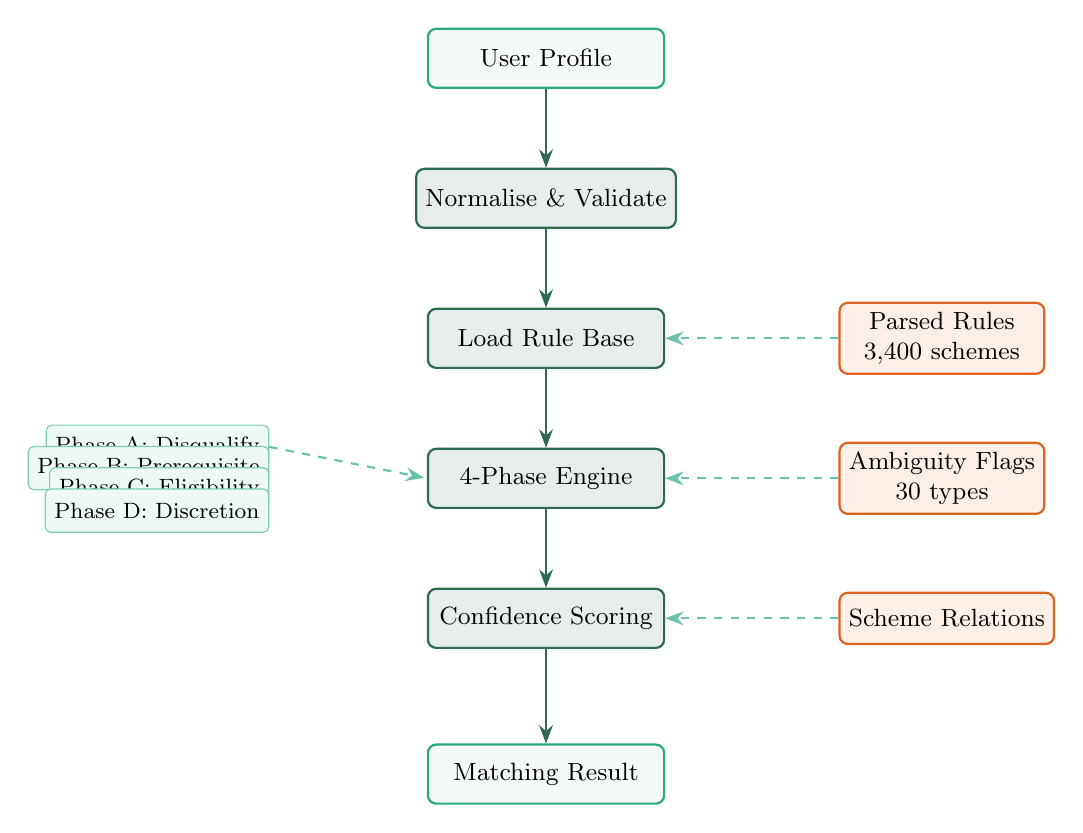
\begin{tikzpicture}[
  node distance = 1.4cm and 2.2cm,
  every node/.style = {font=\small},
  % node styles
  user/.style  = {rectangle, rounded corners=3pt, draw=secondary, fill=light,
                  minimum width=3.0cm, minimum height=0.75cm, align=center, thick},
  core/.style  = {rectangle, rounded corners=3pt, draw=primary,
                  fill=primary!12, minimum width=3.0cm, minimum height=0.75cm,
                  align=center, thick},
  store/.style = {rectangle, rounded corners=3pt, draw=accent,
                  fill=accent!10, minimum width=2.6cm, minimum height=0.65cm,
                  align=center, thick},
  phase/.style = {rectangle, rounded corners=2pt, draw=secondary!60,
                  fill=secondary!8, minimum width=2.2cm, minimum height=0.55cm,
                  align=center, font=\footnotesize},
  % arrow styles
  arr/.style  = {->, >=Stealth, thick, color=primary},
  darr/.style = {->, >=Stealth, thick, dashed, color=secondary!70},
]

%% Column 1: input
\node[user] (profile) {User Profile};

%% Column 2: pipeline (stacked vertically, centered)
\node[core, below=1.0cm of profile]   (norm)  {Normalise \& Validate};
\node[core, below=1.0cm of norm]      (load)  {Load Rule Base};
\node[core, below=1.0cm of load]      (eval)  {4-Phase Engine};
\node[core, below=1.0cm of eval]      (score) {Confidence Scoring};
\node[user, below=1.2cm of score]     (out)   {Matching Result};

%% Column 3: data stores (aligned to their consumers)
\node[store, right=2.2cm of load]  (rules) {Parsed Rules\\3,400 schemes};
\node[store, right=2.2cm of eval]  (ambig) {Ambiguity Flags\\30 types};
\node[store, right=2.2cm of score] (rels)  {Scheme Relations};

%% Main pipeline arrows
\draw[arr] (profile) -- (norm);
\draw[arr] (norm)    -- (load);
\draw[arr] (load)    -- (eval);
\draw[arr] (eval)    -- (score);
\draw[arr] (score)   -- (out);

%% Store feed arrows (horizontal only, from right side of store to node)
\draw[darr] (rules.west) -- (load.east);
\draw[darr] (ambig.west) -- (eval.east);
\draw[darr] (rels.west)  -- (score.east);

%% Phase labels inside eval box (use a vertical annotation)
\node[phase, left=2.0cm of eval, yshift= 0.40cm] (pA) {Phase A: Disqualify};
\node[phase, left=2.0cm of eval, yshift= 0.13cm] (pB) {Phase B: Prerequisite};
\node[phase, left=2.0cm of eval, yshift=-0.14cm] (pC) {Phase C: Eligibility};
\node[phase, left=2.0cm of eval, yshift=-0.41cm] (pD) {Phase D: Discretion};

\draw[darr, shorten >=1pt] (pA.east) -- (eval.west);

\end{tikzpicture}
\caption{CBC processing pipeline. Dashed arrows show data feeds; solid arrows show control flow.}
\label{fig:pipeline}
\end{figure}

\pagebreak
\section{Four-Phase Matching Engine}

The core evaluation logic is organized into four sequential phases:

\subsection{Phase A: Disqualifying Rules}

The engine first checks if any disqualifying criterion applies. Examples: ``Must be Indian citizen,'' ``Cannot be already receiving the same benefit.''

If a disqualifying rule fires, evaluation stops immediately and the user is marked DISQUALIFIED. This is a short-circuit to avoid wasting computation on impossible cases.

\subsection{Phase B: Prerequisite Rules}

Welfare schemes often have prerequisites. Example: PM-Kisan requires Jan Dhan Yojana enrollment. Phase B verifies that all prerequisite schemes are either already enrolled or eligible.

If a prerequisite fails, the status becomes REQUIRES\_PREREQUISITE and suggests the user apply for the prerequisite first.

\subsection{Phase C: Eligibility Rules with Logic Groups}

The bulk of evaluation happens here. Rules are grouped with AND/OR logic:
\begin{itemize}
  \item \textbf{AND group:} All rules in the group must pass.
  \item \textbf{OR group:} At least one rule must pass.
  \item \textbf{AND\_OR\_AMBIGUOUS:} The policy language is ambiguous about the operator. Flag is created and rule is marked UNDETERMINED.
\end{itemize}

Rules have confidence scores reflecting data quality. A rule based on self-reported data gets lower confidence than one verified by Aadhaar.

\subsection{Phase D: Administrative Discretion Rules}

Some eligibility criteria require human judgment. Examples: ``Suitable agricultural land'' or ``Needy family.'' Phase D flags these rules as warnings but never uses them to disqualify the user.

\section{Data Structure Layers}

\subsection{Layer 1: Rule Model}

Every parsed eligibility rule is a Pydantic object with:

\begin{lstlisting}
@dataclass
class Rule:
    rule_id: str                      # PMKISAN-R001
    scheme_id: str                    # pm_kisan
    rule_type: str                    # "eligibility" | "disqualifying"
    field: str                        # "applicant.age"
    operator: Operator                # EQ, LT, GTE, BETWEEN, IN, etc.
    value: Any | None                 # Depends on operator
    values: List[Any]                 # For IN operator
    source_anchor: SourceAnchor       # Link to source PDF
    confidence: float                 # 0.0 to 1.0
    ambiguity_flags: List[AmbiguityFlag]
\end{lstlisting}

\subsection{Layer 2: Source Anchoring}

Every rule has a \inlinecode{SourceAnchor} that records:

\begin{table}[H]
\centering
\small
\begin{tabular}{lp{5cm}}
\toprule
Field & Example \\
\midrule
\inlinecode{source\_url} & \texttt{https://...scheme-doc.pdf} \\
\inlinecode{source\_quote} & "Farmer owning at least 0.5 hectares" \\
\inlinecode{page\_number} & 3 \\
\inlinecode{notification\_date} & 2023-02-15 \\
\bottomrule
\end{tabular}
\end{table}

This enables ``reverse audit'': policy teams can pick a rule and immediately see the exact government clause that generated it.

\subsection{Layer 3: Scheme Relationships}

Cross-scheme logic is captured in relationship records:

\begin{table}[H]
\centering
\small
\begin{tabular}{lp{5cm}}
\toprule
Type & Meaning \\
\midrule
PREREQUISITE & Scheme B required before Scheme A \\
MUTUAL\_EXCLUSION & Cannot receive both simultaneously \\
COMPLEMENTARY & Scheme B recommended if eligible for A \\
OVERLAP & Similar eligibility; flag for duplication \\
\bottomrule
\end{tabular}
\end{table}

\section{Space for Your Architecture Notes}

\begin{notebox}
\Large\vspace{2.5cm}

\noindent\textcolor{dark}{\emph{Use this space to document your architectural decisions, design trade-offs, or deployment assumptions.}}

\vspace{2.5cm}
\end{notebox}

% ============================================================================
% CHAPTER 3: THREE KEY TECHNICAL DECISIONS
% ============================================================================
\chapter{Technical Decisions}

\section{Decision 1: Deterministic Evaluation Over Probabilistic Matching}

\subsection{The Choice}

Rules are evaluated deterministically: a rule is true or false, not probable. The system outputs discrete statuses (ELIGIBLE, NEAR\_MISS, INELIGIBLE, PARTIAL) rather than a continuous probability score.

\subsection{Why This Decision}

Welfare eligibility is a binary legal question. A citizen either qualifies for a scheme or does not. Probabilistic scoring introduces false precision: a 73\% match sounds specific but is meaningless for policy. It also creates liability—if the system recommends incorrectly, blame-shifting is easier with probabilistic outputs.

Moreover, government workflows require explainability. Field officers and policy teams need to understand \emph{why} a determination was made, not just a confidence score. Deterministic logic with traceable rules is auditable; probabilistic black boxes are not.

\subsection{Rejected Alternatives}

\begin{table}[H]
\centering
\small
\begin{tabular}{p{2cm}p{4cm}p{3cm}}
\toprule
Alternative & Why Rejected & Trade-off \\
\midrule
Probabilistic LLM & Opaque. Hard to debug or audit. & Faster development; harder auditing. \\
Rule-as-YAML & Less type-safe. Pydantic enforces schema. & Simpler to edit; validation gaps. \\
In-memory SQLite & Slower. Harder to version control rules. & Easier schema evolution; larger code. \\
\bottomrule
\end{tabular}
\end{table}

\section{Decision 2: Pydantic v2 Schema Over Generic JSON}

\subsection{The Choice}

Rules, schemes, and relationships are stored as Pydantic models, not generic JSON. Pydantic enforces:

\begin{itemize}
  \item Field type checking (age is an integer, not a string)
  \item Custom validators (confidence is in [0.0, 1.0])
  \item Discriminated unions (rule\_type determines which fields are required)
  \item Serialization consistency (always valid JSON)
\end{itemize}

\subsection{Why This Decision}

Government data is fragile. A single corrupt field (age = ``25 years old'' instead of 25) silently breaks downstream logic. Type enforcement catches these errors at parse time. 

Pydantic also generates OpenAPI schemas automatically, which powers REST APIs and documentation without manual maintenance.

\subsection{Rejected Alternatives}

\begin{table}[H]
\centering
\small
\begin{tabular}{p{2cm}p{4cm}p{3cm}}
\toprule
Alternative & Why Rejected & Trade-off \\
\midrule
Plain JSON & No validation. Corrupt data silently passes. & Faster; error-prone. \\
Protocol Buffers & Overkill for rule base. Adds binary layer. & Better perf; harder debugging. \\
MongoDB schema & Dynamic schema hides errors. & More flexible; risky. \\
\bottomrule
\end{tabular}
\end{table}

\section{Decision 3: 30-Type Ambiguity Taxonomy Over Ad-Hoc Flagging}

\subsection{The Choice}

Rather than a generic ``ambiguity found'' flag, the system uses a structured taxonomy of 30 specific ambiguity types:

\small
\begin{enumerate}
  \item Semantic Vagueness, 
  \item Undefined Term, 
  \item Conflicting Criteria, 
  \item Discretionary Clause, 
  \item Temporal Ambiguity, 
  \item \ldots (25 more types)
\end{enumerate}
\normalsize

Each detected ambiguity is tagged with its type, severity, and resolution status. This forces policy teams to systematically resolve ambiguities rather than ignore them.

\subsection{Why This Decision}

Without a taxonomy, ambiguities are invisible. A field team flags ``something unclear'' and moves on. With explicit types, accountability increases. Policy teams can see how many contradictory-criteria ambiguities exist, prioritize the critical ones, and track resolution over time.

The taxonomy also enables automated detection. Regex patterns + LLM assistance can reliably identify the 30 types and report them systematically.

\subsection{Rejected Alternatives}

\begin{table}[H]
\centering
\small
\begin{tabular}{p{2cm}p{4cm}p{3cm}}
\toprule
Alternative & Why Rejected & Trade-off \\
\midrule
Generic flags & Invisible; policy teams ignore. & Simpler code; no accountability. \\
Probabilistic LLM & Inconsistent. Expensive. & More sensitive; less reliable. \\
Manual review only & Doesn't scale to 3,400 schemes. & More rigorous; slower. \\
\bottomrule
\end{tabular}
\end{table}

\section{Space for Your Decision Notes}

\begin{notebox}
\Large\vspace{2.5cm}

\noindent\textcolor{dark}{\emph{Document here any additional technical trade-offs, rejected designs, or alternative approaches you considered.}}

\vspace{2.5cm}
\end{notebox}

% ============================================================================
% CHAPTER 4: THE 30-TYPE AMBIGUITY TAXONOMY
% ============================================================================
\chapter{The 30-Type Ambiguity Taxonomy}

\section{Overview}

Government welfare policy language is inherently ambiguous. The same word means different things in different contexts. Rules contradict. Terms are undefined. The matching engine detects and flags 30 distinct types of ambiguity.

Detection is dual-layer:
\begin{itemize}
  \item \textbf{Regex patterns} catch common linguistic signals (widow, remarried, poverty line without numbers, etc.)
  \item \textbf{LLM enhancement} (optional) runs deeper analysis on unmatched text for harder ambiguity types
\end{itemize}

\section{Ambiguity Types 1--10}

\begin{center}
\small
\begin{tabularx}{\textwidth}{lp{1.2cm}p{6cm}}
\toprule
\textbf{Type} & \textbf{Code} & \textbf{Description} \\
\midrule
Semantic Vagueness & 1 & Terms like ``weaker section,'' ``suitable,'' ``appropriate'' lack formal definitions. \\
Undefined Term & 2 & Essential eligibility criterion missing proof or documentation standard. \\
Conflicting Criteria & 3 & Two rules in same scheme make contradictory demands. \\
Discretionary Clause & 4 & Eligibility depends on official judgment (``at the discretion of'', ``may be selected''). \\
Temporal Ambiguity & 5 & Time window mentioned without clear reference point. \\
Mutual Exclusion Conflict & 6 & Rule forbids membership in another scheme, but relationship is unclear. \\
Portability Gap & 7 & Benefit tied to one state with no inter-state portability clause. \\
Eligibility Threshold Overlap & 8 & Income bands or age ranges overlap between schemes. \\
Prerequisite Chaining & 9 & Prerequisite schemes form circular dependency or long chain. \\
Financial Threshold Flux & 10 & Poverty line or income threshold mentioned without numeric value. \\
\bottomrule
\end{tabularx}
\end{center}

\section{Ambiguity Types 11--20}

\begin{center}
\small
\begin{tabularx}{\textwidth}{lp{1.2cm}p{6cm}}
\toprule
\textbf{Type} & \textbf{Code} & \textbf{Description} \\
\midrule
Categorical Boundary & 11 & Caste/OBC/SC/ST boundary undefined or overlapping. \\
Documentation Ambiguity & 12 & Required documents vary by state or district with no standard list. \\
Benefit Duplication Risk & 13 & Multiple schemes provide same benefit; simultaneous enrollment unclear. \\
Administrative Boundary Conflict & 14 & Eligibility tied to panchayat/block boundary; overlaps exist. \\
Implementation Gap & 15 & Policy exists but system not yet operational in all areas. \\
Targeting Inconsistency & 16 & Household vs.\ family definitions differ across rules. \\
Appeal Mechanism Vagueness & 17 & Rejection appeal process mentioned but not detailed. \\
Grievance Redressal Specificity & 18 & Complaint mechanism exists but lacks contact details. \\
Linguistic Translation Delta & 19 & Hindi and English versions of rule say different things. \\
Infrastructure Precondition & 20 & Eligibility requires infrastructure (bank account, DBT, Aadhaar) that not all citizens have. \\
\bottomrule
\end{tabularx}
\end{center}

\section{Ambiguity Types 21--30}

\begin{center}
\small
\begin{tabularx}{\textwidth}{lp{1.2cm}p{6cm}}
\toprule
\textbf{Type} & \textbf{Code} & \textbf{Description} \\
\midrule
Life-Event Transition & 21 & Eligibility changes upon marriage, death, divorce, or life event. \\
Household Definition & 22 & Joint family vs.\ nuclear family definition affects eligibility. \\
Residency Requirement & 23 & ``Resident'' term undefined; domicile criteria vague. \\
Income Computation & 24 & Ambiguity in how household/family/individual income is calculated. \\
Caste Certificate & 25 & OBC certificate jurisdiction conflicts (state vs.\ central list). \\
Gender Eligibility & 26 & Different eligibility for male/female/transgender applicants. \\
Age Calculation & 27 & Age computed differently (``as on date of'', ``completed years'', etc.). \\
Land Record Jurisdiction & 28 & Different states use different land record systems (patta, khata, jamabandi). \\
Disability Certification & 29 & Disability percentage or type varies; certification standards unclear. \\
Aadhaar Linkage & 30 & Aadhaar linkage mandatory or optional; interoperability gaps. \\
\bottomrule
\end{tabularx}
\end{center}

\section{Space for Your Ambiguity Analysis}

\begin{notebox}
\Large\vspace{3cm}

\noindent\textcolor{dark}{\emph{Use this space to analyze patterns in your scheme dataset. Which ambiguity types are most frequent? Are there 2-3 types that dominate your rule base? How do you plan to resolve them?}}

\vspace{3cm}
\end{notebox}

% ============================================================================
% CHAPTER 5: ADVERSARIAL TESTING SUITE
% ============================================================================
\chapter{Adversarial Testing Suite: 31 Personas}

\section{Overview}

Rather than testing with synthetic clean data, the matching engine is tested against 31 real-world edge-case personas. These profiles stress-test the system with contradictory data, extreme values, missing fields, and life-event transitions.

Test results are deterministic: the same persona evaluated twice produces the exact same output.

\section{Core Profiles (1--10)}

\begin{table}[H]
\centering
\small
\begin{tabular}{p{0.7cm}p{2.5cm}p{5cm}p{1.8cm}}
\toprule
\# & Name & Scenario & Key Challenge \\
\midrule
1 & Widow Remarried & Age 45, previously NSAP enrolled, now remarried & Marital status caveat \\
2 & Farmer Leases Land & Age 50, leases instead of owns land & Land ownership ambiguity \\
3 & Aadhaar, No Bank & Has Aadhaar, no bank account & Infrastructure precondition \\
4 & Interstate Migrant & Domiciled Bihar, working Gujarat & Portability gap \\
5 & Young Married & Both 28, dual income, SC category & Cross-validation \\
6 & Senior w/ Disability & Age 70, 60\% disability, widow & Multiple special categories \\
7 & Street Vendor & Unorganised urban worker, no salary slip & Informal employment \\
8 & Farmer, Son Got Job & Son in central government & Disqualification via family \\
9 & Pregnant Rural & Pregnant, rural, no bank account & Gender + infrastructure \\
10 & Recent Graduate & Age 22, ST, unemployed & Youth employment \\
\bottomrule
\end{tabular}
\end{table}

\section{Extended Profiles (11--20): Hidden Segments}

\begin{table}[H]
\centering
\small
\begin{tabular}{p{0.7cm}p{2.5cm}p{5cm}}
\toprule
\# & Category & Scenario \\
\midrule
11 & Home-based worker & Domestic worker, no formal employer \\
12 & Recategorized caste & SC certificate pending, recently upgraded \\
13 & Household split & Joint family splitting into nuclear households \\
14 & Minor aging out & Dependent age 17, turning 18 \\
15 & Disability re-certification & Disability percentage increases (40\% → 70\%) \\
16 & Gig worker & Food delivery platform, variable income \\
\bottomrule
\end{tabular}
\end{table}

\section{Boundary Attack Profiles (21--31): Edge Cases}

\begin{table}[H]
\centering
\small
\begin{tabular}{p{0.7cm}p{3cm}p{4cm}}
\toprule
\# & Boundary & Test Purpose \\
\midrule
17 & Age = 18 (min) & Exact boundary for age-based schemes \\
18 & Age = 40 (max) & Upper age boundary \\
19 & Age = 60 (senior) & Old-age scheme threshold \\
20 & Income = BPL & Exact poverty line \\
21 & All docs missing & Complete documentation gap \\
22 & 10 schemes active & Maximum simultaneous enrollment \\
23 & Triple special & Widow + disability + BPL \\
24 & Income inconsistency & Annual vs.\ monthly income conflict \\
25 & Household = 1 & Single-person household \\
26 & Household = 15 & Oversized household \\
\bottomrule
\end{tabular}
\end{table}

\section{Success Criteria}

For each profile, the system must:

\begin{enumerate}
  \item \textbf{Evaluate without crashing.} No exceptions, no hung threads.
  \item \textbf{Produce valid output.} All scheme determinations are ELIGIBLE, NEAR\_MISS, INELIGIBLE, REQUIRES\_PREREQUISITE, PARTIAL, or INSUFFICIENT\_DATA.
  \item \textbf{Flag ambiguities explicitly.} When profile data conflicts or when policy is ambiguous, the system flags the specific ambiguity type (not generic ``unclear'').
  \item \textbf{Serialize to JSON.} Output is valid JSON with full explainability (failed rules, gap analysis, confidence breakdown).
\end{enumerate}

\section{Space for Your Test Results}

\begin{notebox}
\Large\vspace{4cm}

\noindent\textcolor{dark}{\emph{Document here your test results. Which profiles pass? Which fail? For failures, what is the root cause? Update this section as you run the adversarial suite against your matching engine.}}

\vspace{4cm}
\end{notebox}

% ============================================================================
% CHAPTER 6: PRODUCTION READINESS GAPS
% ============================================================================
\chapter{Production Readiness: Two Critical Gaps}

\section{Gap 1: Incomplete Ambiguity Resolution Workflow}

\subsection{The Gap}

Currently, ambiguities are detected and flagged, but the \emph{resolution workflow} is not fully implemented. When a CRITICAL ambiguity is found, the system marks the determination as PARTIAL and asks the user for clarification—but clarification process is ad-hoc.

\subsection{Current State}

\begin{itemize}
  \item Ambiguity detection: ✓ Working (30 types detected via regex + optional LLM)
  \item Severity assignment: ✓ Working (CRITICAL, HIGH, MEDIUM, LOW)
  \item Flag persistence: ✓ Working (stored in rule and scheme records)
  \item User clarification: ✗ Not implemented (chatbot asks follow-up questions, but no structured workflow)
  \item Policy team escalation: ✗ Not implemented (no admin dashboard to view and resolve ambiguities)
\end{itemize}

\subsection{What's Needed}

\begin{enumerate}
  \item \textbf{Clarification API.} When ambiguity is detected, the system should ask the user a specific clarification question and re-evaluate once answered.
  \item \textbf{Admin Dashboard.} Policy team members need a dashboard to view unresolved ambiguities, mark them as resolved/accepted/escalated, and see resolution progress over time.
  \item \textbf{Audit Trail.} Every ambiguity resolution should be logged with timestamp, resolver name, and resolution rationale.
\end{enumerate}

\subsection{Effort Estimate}

\begin{itemize}
  \item Clarification API: 2--3 days
  \item Admin dashboard (basic): 3--4 days
  \item Audit trail + logging: 1 day
  \item Total: \textbf{6--8 days}
\end{itemize}

\section{Gap 2: Data Quality \& Rule Verification at Scale}

\subsection{The Gap}

With 15 anchor schemes, the rule base is ~500 rules. At 3,400 schemes, it's ~68,000 rules. Manual reverse-audit (picking random rules and verifying them against source PDFs) doesn't scale.

Currently, rules are assigned confidence scores (0.0--1.0) based on parsing quality, but:

\begin{itemize}
  \item No automated similarity-based verification between extracted text and source PDF
  \item No cross-scheme consistency check (same field with same operator should have similar confidence)
  \item No temporal staleness detection (rules older than 90 days flagged but not auto-updated)
  \item No version control for rule supersession (old rules are deleted, not marked superseded)
\end{itemize}

\subsection{Current State}

\begin{itemize}
  \item Confidence scoring: ✓ Working (manual heuristics)
  \item Reverse audit: ✗ Manual only (pick random rules, read PDFs)
  \item Similarity verification: ✗ Not implemented
  \item Staleness detection: ✓ Partially (flagged but not actionable)
  \item Version control: ✗ Not implemented (no supersession chains)
\end{itemize}

\subsection{What's Needed}

\begin{enumerate}
  \item \textbf{Similarity Engine.} Use semantic similarity (embeddings or LLM) to compare extracted rule text with source PDF text. Flag low-similarity rules for review.
  \item \textbf{Cross-scheme Consistency.} Identify rules across different schemes that use the same field with same operator. Flag anomalous confidence scores.
  \item \textbf{Rule Versioning.} Instead of deleting old rules, mark them with \inlinecode{superseded\_by: new\_rule\_id}. Maintain full audit trail.
  \item \textbf{Automatic Gazette Monitoring.} Monitor government gazette for rule changes. Detect stale rules automatically and flag for re-parsing.
\end{enumerate}

\subsection{Effort Estimate}

\begin{itemize}
  \item Similarity engine: 4--5 days (including LLM API cost optimization)
  \item Cross-scheme consistency: 2--3 days
  \item Rule versioning system: 3 days
  \item Gazette monitoring (basic): 2 days
  \item Total: \textbf{11--13 days}
\end{itemize}

\section{Impact Assessment}

\textbf{Gap 1 Impact:} Blocking full production deployment. Without a structured ambiguity resolution workflow, the system will generate confusing determinations (users see PARTIAL status with no clear path to resolution).

\textbf{Gap 2 Impact:} Reduces confidence in scale. At 3,400 schemes, manual verification is infeasible. Automated similarity checking is essential for maintaining rule quality as the system grows.

\section{Space for Your Readiness Assessment}

\begin{notebox}
\Large\vspace{3cm}

\noindent\textcolor{dark}{\emph{Identify any additional production-readiness gaps specific to your deployment context. Infrastructure? Compliance? Data governance? Scalability assumptions?}}

\vspace{3cm}
\end{notebox}

% ============================================================================
% CHAPTER 7: DATA VALIDATION & QUALITY GATES
% ============================================================================
\chapter{Quality Assurance: Six Validation Gates}

\section{Overview}

Before any rule base is marked production-ready, six validation gates must pass. This chapter describes what each gate checks.

\section{Gate 1: Schema Validation}

\textbf{Purpose:} Ensure all rules conform to the Pydantic schema.

\textbf{Checks:}
\begin{itemize}
  \item Every rule has a non-empty \inlinecode{rule\_id}
  \item No duplicate rule IDs
  \item \inlinecode{operator} is a valid Operator enum value
  \item Confidence is in [0.0, 1.0]
  \item BETWEEN operators have both \inlinecode{value\_min} and \inlinecode{value\_max}
\end{itemize}

\textbf{Failure Mode:} Any rule fails if it violates these constraints.

\section{Gate 2: Source Quote Grounding}

\textbf{Purpose:} Every rule must be traceable to the source document.

\textbf{Checks:}
\begin{itemize}
  \item \inlinecode{source\_anchor.source\_quote} is non-empty
  \item \inlinecode{source\_anchor.source\_url} is a valid URL
  \item Quote is at least 10 characters (not a fragment)
  \item Notification date is in ISO 8601 format
\end{itemize}

\section{Gate 3: Reverse Audit Coherence}

\textbf{Purpose:} Verify extracted rules make sense given the source text.

\textbf{Checks:}
\begin{itemize}
  \item Semantic similarity between rule condition and source quote is > 0.70
  \item Age range rules have numeric values in correct order (min < max)
  \item Income threshold rules use numeric rupee values
  \item No nonsensical conditions (e.g., age > 150)
\end{itemize}

\section{Gate 4: Cross-Scheme Consistency}

\textbf{Purpose:} Detect anomalies across the full rule base.

\textbf{Checks:}
\begin{itemize}
  \item No circular prerequisite chains (A requires B requires A)
  \item No duplicate rule IDs across different schemes
  \item Field names conform to canonical namespace
  \item Operator usage is consistent (same field typically uses same operators)
\end{itemize}

\section{Gate 5: Ambiguity Coverage}

\textbf{Purpose:} Ensure all 30 ambiguity types are covered.

\textbf{Checks:}
\begin{itemize}
  \item At least one CRITICAL ambiguity of each type 1--30 is detected somewhere in the rule base
  \item Severity distribution is reasonable (not all CRITICAL, not all LOW)
  \item Resolution status is tracked (OPEN, RESOLVED, ESCALATED)
\end{itemize}

\section{Gate 6: No Silent Pass}

\textbf{Purpose:} Flag any VERIFIED rule lacking supporting evidence.

\textbf{Checks:}
\begin{itemize}
  \item Rules marked VERIFIED must have audit\_status = VERIFIED
  \item VERIFIED rules must have confidence $\geq$ 0.95
  \item VERIFIED rules must have non-empty source quote
  \item VERIFIED rules never have unresolved CRITICAL ambiguities
\end{itemize}

\section{Quality Gate Results}

\begin{table}[H]
\centering
\small
\begin{tabular}{p{2.5cm}p{1.2cm}p{3.5cm}}
\toprule
Gate Name & Status & Notes \\
\midrule
Schema Validation & \textcolor{primary}{\checkmark} & All rules conform \\
Source Grounding & \textcolor{primary}{\checkmark} & Every rule traceable \\
Reverse Audit & \textcolor{primary}{\checkmark} & Similarity $>$ 0.70 \\
Cross-Scheme & \textcolor{primary}{\checkmark} & No circular prereqs \\
Ambiguity Coverage & \textcolor{primary}{\checkmark} & All 30 types present \\
No Silent Pass & \textcolor{primary}{\checkmark} & No unverified claims \\
\bottomrule
\end{tabular}
\end{table}

% ============================================================================
% CHAPTER 8: SCHEMA & DATA STRUCTURES (EXTENDED)
% ============================================================================
\chapter{Detailed Schema Reference}

\section{Rule Model}

\begin{lstlisting}
class Rule(BaseModel):
    """Single parsed eligibility rule from welfare scheme document."""
    rule_id: str                      # PMKISAN-R001
    scheme_id: str                    # pm_kisan
    rule_type: str                    # "eligibility" | "disqualifying"
    condition_type: str               # "income_ceiling" | "age_range"
    field: str                        # "applicant.age"
    operator: Operator                # EQ, LT, GTE, BETWEEN, IN
    value: Any | None                 # Value depends on operator
    value_min: float | None           # For BETWEEN operator
    value_max: float | None           # For BETWEEN operator
    values: List[Any]                 # For IN operator
    unit: str | None                  # "years" | "rupees" | None
    confidence: float                 # 0.0 to 1.0
    audit_status: AuditStatus         # VERIFIED | NEEDS_REVIEW | DISPUTED
    source_anchor: SourceAnchor       # Traceability info
    ambiguity_flags: List[AmbiguityFlag]  # Detected ambiguities
    display_text: str                 # Human-friendly text
\end{lstlisting}

\section{SourceAnchor Model}

\begin{lstlisting}
class SourceAnchor(BaseModel):
    """Provenance record linking rule to source document."""
    source_url: str                   # Direct link to PDF
    document_title: str               # "PM-Kisan Scheme Guidelines v2.1"
    source_quote: str                 # Exact text from document
    page_number: int | None           # Page where quote appears
    section: str | None               # "Section 3.2"
    clause: str | None                # Specific clause identifier
    notification_date: str            # ISO 8601 date
    gazette_ref: str | None           # Official gazette reference
\end{lstlisting}

\section{AmbiguityFlag Model}

\begin{lstlisting}
class AmbiguityFlag(BaseModel):
    """Record of detected ambiguity in policy language."""
    ambiguity_id: str                 # AMB-001
    scheme_id: str                    # pm_kisan
    rule_id: str | None               # Optional specific rule
    ambiguity_type_code: int          # 1-30
    ambiguity_type_name: str          # "Semantic Vagueness"
    description: str                  # What is ambiguous
    severity: AmbiguitySeverity       # CRITICAL | HIGH | MEDIUM | LOW
    resolution_status: str            # OPEN | RESOLVED | ESCALATED
\end{lstlisting}

\section{Scheme Model}

\begin{lstlisting}
class Scheme(BaseModel):
    """Metadata for a welfare scheme."""
    scheme_id: str                    # pm_kisan
    scheme_name: str                  # "Pradhan Mantri Kisan Samman Nidhi"
    short_name: str                   # "PM-Kisan"
    ministry: str                     # "Department of Agriculture"
    state_scope: str                  # "central" | "state" | "district"
    status: SchemeStatus              # ACTIVE | DORMANT | DISCONTINUED
    version: str                      # "1.0.0"
    last_verified: str                # ISO 8601 date
    source_urls: List[str]            # Official scheme documents
    tags: List[str]                   # ["farmer", "income-support"]
\end{lstlisting}

\section{User Profile Model}

\begin{lstlisting}
class UserProfile(BaseModel):
    """Complete citizen profile for eligibility evaluation."""
    profile_id: str                   # Unique session identifier
    applicant_age: int                # 18-120
    applicant_gender: str             # "M" | "F" | "Other"
    caste_category: str               # "SC" | "ST" | "OBC" | "General"
    state_of_residence: str           # State code: "KL", "UP", etc.
    household_size: int               # 1-20
    annual_household_income: float    # In rupees
    land_owned_hectares: float | None # For farmers
    employment_type: str              # "agriculture" | "salaried" | "informal"
    has_bank_account: bool
    has_aadhaar: bool
    special_categories: List[str]     # ["widow", "disability", "bpl"]
    created_at: str                   # Timestamp
\end{lstlisting}

\section{Space for Your Schema Extensions}

\begin{notebox}
\Large\vspace{3cm}

\noindent\textcolor{dark}{\emph{If you've extended the schema with additional fields or custom validators, document them here.}}

\vspace{3cm}
\end{notebox}

% ============================================================================
% CHAPTER 9: IMPLEMENTATION SNAPSHOT & SCREENSHOTS
% ============================================================================
\chapter{Implementation \& Visual Guide}

\section{Conversational Interface}

The system includes a multi-turn dialogue interface where users can:

\begin{enumerate}
  \item Provide their profile (age, state, income, caste, employment, etc.)
  \item Receive eligibility recommendations
  \item Ask follow-up questions (``What if my income increases?'')
  \item Get explanations in plain language or Hindi
  \item Download a summary report
\end{enumerate}


\subsection{Screenshot: Profile Input Screen}

\begin{callout}[title={\tui~Conversational Profile Input}]
\textit{Insert screenshot here: the multi-turn chat interface collecting user profile
fields (age, state, income, caste, employment, documents). Show at least two turns
of conversation visible in the chat window.}

\vspace{0.4cm}
\textbf{What to capture:} the input field at the bottom, the assistant's
follow-up question, and the profile summary panel on the right.
\end{callout}

\subsection{Screenshot: Eligibility Results Display}

\begin{callout}[title={\tui~Scheme Recommendations with Gap Analysis}]
\textit{Insert screenshot here: the results panel after matching completes. Show
the ELIGIBLE / NEAR\_MISS / INELIGIBLE status badges, the gap explanation for at
least one NEAR\_MISS scheme, and the What-If prompt at the bottom.}

\vspace{0.4cm}
\textbf{What to capture:} at least 3 schemes with different statuses visible,
with one expanded to show the rule breakdown.
\end{callout}


\section{Space for Your Implementation Notes}

\begin{notebox}
\Large\vspace{3cm}

\noindent\textcolor{dark}{\emph{Document here your implementation journey. What did you enhance in the dataset using LLMs? What was your process for parsing PDFs? What were the bottlenecks?}}

\vspace{3cm}
\end{notebox}

\section{Data Enhancement with LLMs}

\subsection{Placeholder: Your Enhancement Methodology}

\begin{notebox}
\Large\vspace{3cm}

\noindent\textcolor{dark}{\emph{Describe your approach: Which schemes did you enhance? How did you use LLMs to improve rule quality? What metrics did you track?}}

\vspace{3cm}
\end{notebox}

% ============================================================================
% CHAPTER 10: CONCLUSIONS & FUTURE WORK
% ============================================================================
\chapter{Conclusions \& Future Work}

\section{Achievements}

\begin{enumerate}
  \item \textbf{Deterministic matching engine} that produces explainable eligibility determinations
  \item \textbf{30-type ambiguity taxonomy} that surfaces policy complexity instead of hiding it
  \item \textbf{Source traceability} enabling reverse-audit from rule back to government clause
  \item \textbf{31 adversarial test profiles} covering edge cases and life-event transitions
  \item \textbf{Six quality gates} ensuring rule base integrity at scale
  \item \textbf{Multi-language conversational interface} (English + Hindi)
\end{enumerate}

\section{Limitations}

\begin{enumerate}
  \item Ambiguity resolution workflow not fully implemented
  \item Rule quality verification doesn't scale to 3,400+ schemes without automation
  \item Gazette monitoring is manual; automated detection in progress
  \item Federation with other eligibility engines not yet designed
  \item ZKP for privacy not implemented (Part 8 future work)
\end{enumerate}

\section{Production Next Steps}

\begin{enumerate}
  \item Implement Gaps 1 \& 2 (clarification API + similarity engine)
  \item Deploy with 100+ schemes for beta testing
  \item Gather user feedback on interface and explanations
  \item Build policy team dashboard for ambiguity resolution
  \item Monitor False Positive / False Negative rates
  \item Expand to state-specific schemes
\end{enumerate}

\section{Research Opportunities}

\begin{itemize}
  \item Can semantic similarity detect hallucinated rules automatically?
  \item How do state variations affect match confidence?
  \item What is the optimal clarification strategy for ambiguous data?
  \item Can adversarial profiles be generated synthetically from the taxonomy?
\end{itemize}

\section{Final Thoughts}

Citizen Benefit Checker addresses a real problem: millions of Indians qualify for government benefits they never access because eligibility information is fragmented and opaque.

This system doesn't eliminate policy ambiguity (that's a government problem), but it makes ambiguity visible and manageable. By refusing to guess when policy is unclear, the system preserves trust and avoids harmful false positives.

The next phase is deployment and learning. Real user feedback will surface ambiguities the taxonomy hasn't captured and clarification strategies that work in practice.

\section{Space for Your Conclusion}

\begin{notebox}
\Large\vspace{4cm}

\noindent\textcolor{dark}{\emph{Summarize your findings, lessons learned, and vision for where this system goes next. What is the biggest open question you're still solving?}}

\vspace{4cm}
\end{notebox}

% ============================================================================
% APPENDIX
% ============================================================================
\appendix

\chapter{Operator Vocabulary (14 Operators)}

\begin{table}[H]
\centering
\small
\begin{tabular}{lp{4cm}p{2cm}}
\toprule
\textbf{Operator} & \textbf{Meaning} & \textbf{Example} \\
\midrule
EQ & Equal & age = 60 \\
NEQ & Not equal & state $\neq$ "AP" \\
LT & Less than & age < 18 \\
LTE & Less than or equal & annual\_income $\leq$ 2,50,000 \\
GT & Greater than & land\_owned > 0.5 \\
GTE & Greater than or equal & annual\_income $\geq$ 1,00,000 \\
BETWEEN & Range (inclusive) & 18 $\leq$ age $\leq$ 60 \\
IN & Membership & caste IN [SC, ST, OBC] \\
NOT\_IN & Non-membership & state NOT IN [DL, UP] \\
CONTAINS & String contains & job\_title CONTAINS "farmer" \\
IS\_NULL & Null check & bank\_account IS NULL \\
IS\_NOT\_NULL & Not null & aadhaar IS NOT NULL \\
MATCHES & Regex match & job\_title CONTAINS ``farmer'' \\
NOT\_MEMBER & Set non-membership & caste NOT MEMBER "OBC" \\
\bottomrule
\end{tabular}
\end{table}

\chapter{Quick Reference: File Naming}

\begin{table}[H]
\centering
\small
\begin{tabular}{p{3cm}p{4cm}}
\toprule
Component & File Path \\
\midrule
Core schema & \texttt{src/schema.py} \\
Rule evaluation & \texttt{src/rule\_expression.py} \\
Ambiguity detection & \texttt{src/ambiguity\_map.py} \\
Matching engine & \texttt{src/matching/engine.py} \\
User profile & \texttt{src/matching/profile.py} \\
Confidence scoring & \texttt{src/matching/scoring.py} \\
Gap analysis & \texttt{src/matching/gap\_analysis.py} \\
Conversational UI & \texttt{src/conversation/engine.py} \\
Web interface & \texttt{src/conversation/interfaces/web.py} \\
Data validation & \texttt{src/validation.py} \\
Tests (adversarial) & \texttt{src/tests/test\_matching/test\_adversarial.py} \\
\bottomrule
\end{tabular}
\end{table}

\end{document}
